% Für Bindekorrektur als optionales Argument "BCORfaktormitmaßeinheit", dann
% sieht auch Option "twoside" vernünftig aus
% Näheres zu "scrartcl" bzw. "scrreprt" und "scrbook" siehe KOMA-Skript Doku
\documentclass[12pt,a4paper,titlepage,headinclude,bibtotoc]{scrartcl}


%---- Allgemeine Layout Einstellungen ------------------------------------------

% Für Kopf und Fußzeilen, siehe auch KOMA-Skript Doku
\usepackage[komastyle]{scrpage2}
\pagestyle{scrheadings}
\automark[section]{chapter}
\setheadsepline{0.5pt}[\color{black}]

%keine Einrückung
\parindent0pt

%Einstellungen für Figuren- und Tabellenbeschriftungen
\setkomafont{captionlabel}{\sffamily\bfseries}
\setcapindent{0em}

\usepackage{caption}

%---- Weitere Pakete -----------------------------------------------------------
% Die Pakete sind alle in der TeX Live Distribution enthalten. Wichtige Adressen
% www.ctan.org, www.dante.de

% Sprachunterstützung
\usepackage[ngerman]{babel}

% Benutzung von Umlauten direkt im Text
% entweder "latin1" oder "utf8"
\usepackage[utf8]{inputenc}

% Pakete mit Mathesymbolen und zur Beseitigung von Schwächen der Mathe-Umgebung
\usepackage{latexsym,exscale,amssymb,amsmath}

% Weitere Symbole
\usepackage[nointegrals]{wasysym}
\usepackage{eurosym}

% Anderes Literaturverzeichnisformat
%\usepackage[square,sort&compress]{natbib}

% Für Farbe
\usepackage{color}

% Zur Graphikausgabe
%Beipiel: \includegraphics[width=\textwidth]{grafik.png}
\usepackage{graphicx}

% Text umfließt Graphiken und Tabellen
% Beispiel:
% \begin{wrapfigure}[Zeilenanzahl]{"l" oder "r"}{breite}
%   \centering
%   \includegraphics[width=...]{grafik}
%   \caption{Beschriftung} 
%   \label{fig:grafik}
% \end{wrapfigure}
\usepackage{wrapfig}

% Mehrere Abbildungen nebeneinander
% Beispiel:
% \begin{figure}[htb]
%   \centering
%   \subfigure[Beschriftung 1\label{fig:label1}]
%   {\includegraphics[width=0.49\textwidth]{grafik1}}
%   \hfill
%   \subfigure[Beschriftung 2\label{fig:label2}]
%   {\includegraphics[width=0.49\textwidth]{grafik2}}
%   \caption{Beschriftung allgemein}
%   \label{fig:label-gesamt}
% \end{figure}
\usepackage{subfigure}
\usepackage{adjustbox}

% Caption neben Abbildung
% Beispiel:
% \sidecaptionvpos{figure}{"c" oder "t" oder "b"}
% \begin{SCfigure}[rel. Breite (normalerweise = 1)][hbt]
%   \centering
%   \includegraphics[width=0.5\textwidth]{grafik.png}
%   \caption{Beschreibung}
%   \label{fig:}
% \end{SCfigure}
\usepackage{sidecap}

% Befehl für "Entspricht"-Zeichen
\newcommand{\corresponds}{\ensuremath{\mathrel{\widehat{=}}}}

%Für chemische Formeln (von www.dante.de)
%% Anpassung an LaTeX(2e) von Bernd Raichle
\makeatletter
\DeclareRobustCommand{\chemical}[1]{%
  {\(\m@th
   \edef\resetfontdimens{\noexpand\)%
       \fontdimen16\textfont2=\the\fontdimen16\textfont2
       \fontdimen17\textfont2=\the\fontdimen17\textfont2\relax}%
   \fontdimen16\textfont2=2.7pt \fontdimen17\textfont2=2.7pt
   \mathrm{#1}%
   \resetfontdimens}}
\makeatother

%Si Einheiten
\usepackage{siunitx}

%c++ Code einbinden
\usepackage{listings}
\lstset{numbers=left, numberstyle=\tiny, numbersep=5pt}

%Differential
\newcommand{\dif}{\ensuremath{\mathrm{d}}}

%Boxen,etc.
\usepackage{fancybox}
\usepackage{empheq}

%Fußnoten auf gleiche Seite
\interfootnotelinepenalty=1000

%Dateien aus Unterverzeichnissen
\usepackage{import}

%Bibliography \bibliography{literatur} und \cite{gerthsen}
%\usepackage{cite}
\usepackage{babelbib}
\selectbiblanguage{ngerman}

\begin{document}

\begin{titlepage}
\centering
\textsc{\Large Anfängerpraktikum der Fakultät für
  Physik,\\[1.5ex] Universität Göttingen}

\vspace*{4.2cm}

\rule{\textwidth}{1pt}\\[0.5cm]
{\huge \bfseries
  Messung von großen Widerständen\\[1.5ex]
  Protokoll:}\\[0.5cm]
\rule{\textwidth}{1pt}

\vspace*{3.0cm}

\begin{Large}
\begin{tabular}{ll}
Praktikant:
 	&  Felix Kurtz\\
 	&  Michael Lohmann\\

E-Mail: 
	&  felix.kurtz@stud.uni-goettingen.de\\
	& m.lohmann@stud.uni-goettingen.de\\

 Betreuer: & Björn Klaas\\
 Versuchsdatum: &  03.09.2014\\
\end{tabular}
\end{Large}

\vspace*{0.8cm}

\begin{Large}
\fbox{
  \begin{minipage}[t][2.5cm][t]{6cm} 
    Testat:
  \end{minipage}
}
\end{Large}

\end{titlepage}

\tableofcontents

\newpage

\section{Einleitung}
\label{sec:einleitung}
Um einen Widerstand zu messen, nutzt man meistens das Ohmsche Gesetz.
Ist der Widerstand jedoch hochohmig, stößt dieses Verfahren an seine Grenzen.
Man arbeitet mit hohen Spannungen und kleinen Strömen.
Außerdem sind die Innenwiderstände der Messgeräte ein großer Störfaktor.
Deshalb werden wir in diesem Versuch lernen, wie man das besser machen kann. 

\section{Theorie}
\label{sec:theorie}
\subsection{Messung mittels einem Kondensator}

\begin{align}
	Q(t)=Q_0 \exp \left(-\frac{t}{RC}\right)
	\label{eq:Q(t)}
\end{align}
Kennt man die Kapazität $C$ und die Ladung, die sich auf dem Kondensator befindet, zu zwei verschiedenen Zeitpunkten $t_1$ und $t_2$, kann man also den Widerstand $R$ berechnen, über den der Strom abfließt:
\begin{align}
	R=-\frac{t_2-t_1}{C\cdot\ln\frac{Q(t_2)}{Q(t_1)}}
\end{align}
Der hier verwendete Kondenstor hat einen Plattenradius $r=0.1~\si{\meter}$, einen Plattenabstand $d=0.005~\si{\meter}$ und eine Plattenzahl $n=65$.
Für die Berechnung der Kapazität müssen also Randeffekte betrachtet werden.
Dabei wird diese Formel verwendet:
\begin{align}	
	C_n=(n-1)\varepsilon_0\varepsilon_r\left[\frac{\pi r^2}{d}+r\left(\ln\frac{16\pi r}{d}-1\right)\right]
	\label{eq:C_Pl}
\end{align}
%ergibt sich eine Kapazität $C=3.896~\si{\nano\farad}$.

\subsection{Analoger Stromintegrator}
Nach der \textit{Kirchhoffschen Knotenregel} bei S gilt $I_R+I_C=0$.
Mit den folgenden Beziehungen der Ströme $I_R=U_E/R$ und $I_C=\dot{Q}_C=C\dot{U}_A$ erhält man:
\begin{align}
	U_A=-\frac{1}{RC}\int \limits_{t_0}^t U_E \,\dif t
\end{align}

\subsection{RLC-Schwingkreis}
\begin{align}
	\ddot{Q}+2\beta\dot{Q}+\omega_0^2 Q=0
\end{align}
\begin{align*}
	\beta=\frac{R_L}{2L} \quad , \quad 
	\omega_0=\sqrt{\frac{1}{LC}} \quad , \quad
	\omega=\sqrt{\omega_0^2-\beta^2}
\end{align*}
Mit dem Logarithmischen Dekrement $\Lambda=\beta T$ ergibt sich für die Induktivität der Spule
\begin{align}
	L=\frac{1}{C\omega_0^2}=\frac{1}{C(\omega^2+\beta^2)}=\frac{1}{C}\frac{T^2}{4\pi^2+\Lambda^2}
\end{align}
\begin{align}
	L=\mu_0 \cdot A \cdot \left(\frac{n}{l}\right)^2
\end{align}

\section{Durchführung}
\label{sec:durchfuehrung}
\subsection{Kalibrieren des Ladungsmessgerätes}
Dazu wird der Eichkreis nach Abb. \ref{} verschaltet.
Der Eichgenerator wird in der Stellung \emph{Zeitmessung} mit dem Oszilloskop auf verschiedene Zeitdauern der Spannungsimpulse eingestellt.
Erwartet werden Werte zwischen 50 und 500 Millisekunden.
Je eingestellter Zeitdauer wird dann in der Stellung \emph{Eichen} dreimal der Messwert des Ladungsmessgerätes notiert.
Dies geschieht für 5 verschiedene Zeiten.

\subsection{Entladung des Plattenkondensators}
Der  Plattenkondensator wir mit 220V aufgeladen und sofort durch den Messkreis entladen.
Dabei wird die geflossene Ladung gemessen.
Dies geschieht fünfmal.\\
Nun wird der Kondensator wieder aufgeladen und nach bestimmten Zeiten (t=0, 1,2,3,5 Minuten) über das Ladungsmessgerät entladen.
Die verbleibende Ladung wird notiert.
In der Zwischenzeit ist Ladung über den Isolationswiderstand des Kondensators abgeflossen.
Mit dieser Methode kann man eben diesen bestimmen.\\
Parallel wird der unbekannte Widerstand $R_x$ geschaltet und vorige Messung für folgende Zeiten wiederholt: 0, 2, 4, 6, 8, 10, 20, 30 und 60 Sekunden.
Für jede Zeitspanne werden zwei Werte aufgenommen.

\subsection{Schwingkreise}
Man tauscht im Messkreis das Ladungsmessgerät durch das Oszilloskop.
Dieses soll den Spannungsverlauf $U(t)$ am Kondensator zeigen.
\begin{enumerate}
	\item Plattenkondensator alleine
	\item Kondensator und 2M$\Omega$-Widerstand parallel dazu
	\item Kondensator und Widerstand $R_x$ parallel dazu
	\item Kondensator und Drosselspule parallel
	\item Kondensator und Luftspule parallel
	\item Kommerzieller Kondensator (Folienkondensator) und 2M$\Omega$-Widerstand parallel dazu	
\end{enumerate}
Die vom Oszilloskop angezeigten Spannungsverläufe werden mit dem zugehörigen Drucker ausgedruckt.
Bei Messungen von einem RC-Kreis sollte man die \emph{Abfallzeit} vom Oszilloskop berechnen lassen, also die Zeit, die zwischen $90\%$ und $10\%$ der Maximalspannung vergeht\footnote{aus der Anleitung (S. 29) des verwendeten Oszilloskops TDS 2001C, abgerufen am 09.09.2014:\\ 
\emph{http://www.praktikum.physik.uni-goettingen.de/allgemeines/anleitung/downloads/TDS200E\_71048501.pdf}}.
Dies vereinfacht die Auswertung.
Bei den RLC-Kreisen benötigt man die Periode der abklingenden Schwingung. 
Zur Erzielung guter Ergebnisse mussten wir am Oszilloskop die Einstellung \emph{Tastknopf} auf 50x stellen.

\subsection{Messungen mit dem Multimeter}
Mit dem Multimeter werden folgende Größen gemessen:
\begin{itemize}
	\item ohmsche Widerstände $R_L$ der beiden Spulen
	\item ohmscher Widerstand $R_2$ (2M$\Omega$)
	\item Isolationswiderstand $R_\text{iso}$ des Plattenkondenstaors
	\item unbekannter Widerstand $R_x$
 	\item Kapazitäten $C$ der beiden Kondensatoren  
\end{itemize}
Außerdem werden die Daten der Luftspule an deren Ende abgelesen.

\section{Auswertung}
\label{sec:auswertung}
\subsection{Kalibration des Ladungsmessgerätes}
Um das Ladungsmessgerät zu eichen, lässt man einen konstanten Strom $I$ für eine bestimmte Zeit $t$ fließen.
Es fließt also insgesamt die Ladung $Q=I \cdot t$.
Trägt man also die abgelesen Skalenteile gegen die tatsächliche Ladung auf - wie in Abb.\ref{fig:Kalibration} - kann man nun Skalenteile in Coulomb über die Geradensteigung $m$ umrechnen.
Es ergibt sich:
$$m=0.8729 \pm 0.0017 ~\text{Skt.}/\si{\micro\coulomb}$$
Da der Fehler sehr klein ist, wird er bei den nun folgenden Umrechnungen weggelassen.

\begin{figure}
 \centering
 % GNUPLOT: LaTeX picture with Postscript
\begingroup
  \makeatletter
  \providecommand\color[2][]{%
    \GenericError{(gnuplot) \space\space\space\@spaces}{%
      Package color not loaded in conjunction with
      terminal option `colourtext'%
    }{See the gnuplot documentation for explanation.%
    }{Either use 'blacktext' in gnuplot or load the package
      color.sty in LaTeX.}%
    \renewcommand\color[2][]{}%
  }%
  \providecommand\includegraphics[2][]{%
    \GenericError{(gnuplot) \space\space\space\@spaces}{%
      Package graphicx or graphics not loaded%
    }{See the gnuplot documentation for explanation.%
    }{The gnuplot epslatex terminal needs graphicx.sty or graphics.sty.}%
    \renewcommand\includegraphics[2][]{}%
  }%
  \providecommand\rotatebox[2]{#2}%
  \@ifundefined{ifGPcolor}{%
    \newif\ifGPcolor
    \GPcolortrue
  }{}%
  \@ifundefined{ifGPblacktext}{%
    \newif\ifGPblacktext
    \GPblacktexttrue
  }{}%
  % define a \g@addto@macro without @ in the name:
  \let\gplgaddtomacro\g@addto@macro
  % define empty templates for all commands taking text:
  \gdef\gplbacktext{}%
  \gdef\gplfronttext{}%
  \makeatother
  \ifGPblacktext
    % no textcolor at all
    \def\colorrgb#1{}%
    \def\colorgray#1{}%
  \else
    % gray or color?
    \ifGPcolor
      \def\colorrgb#1{\color[rgb]{#1}}%
      \def\colorgray#1{\color[gray]{#1}}%
      \expandafter\def\csname LTw\endcsname{\color{white}}%
      \expandafter\def\csname LTb\endcsname{\color{black}}%
      \expandafter\def\csname LTa\endcsname{\color{black}}%
      \expandafter\def\csname LT0\endcsname{\color[rgb]{1,0,0}}%
      \expandafter\def\csname LT1\endcsname{\color[rgb]{0,1,0}}%
      \expandafter\def\csname LT2\endcsname{\color[rgb]{0,0,1}}%
      \expandafter\def\csname LT3\endcsname{\color[rgb]{1,0,1}}%
      \expandafter\def\csname LT4\endcsname{\color[rgb]{0,1,1}}%
      \expandafter\def\csname LT5\endcsname{\color[rgb]{1,1,0}}%
      \expandafter\def\csname LT6\endcsname{\color[rgb]{0,0,0}}%
      \expandafter\def\csname LT7\endcsname{\color[rgb]{1,0.3,0}}%
      \expandafter\def\csname LT8\endcsname{\color[rgb]{0.5,0.5,0.5}}%
    \else
      % gray
      \def\colorrgb#1{\color{black}}%
      \def\colorgray#1{\color[gray]{#1}}%
      \expandafter\def\csname LTw\endcsname{\color{white}}%
      \expandafter\def\csname LTb\endcsname{\color{black}}%
      \expandafter\def\csname LTa\endcsname{\color{black}}%
      \expandafter\def\csname LT0\endcsname{\color{black}}%
      \expandafter\def\csname LT1\endcsname{\color{black}}%
      \expandafter\def\csname LT2\endcsname{\color{black}}%
      \expandafter\def\csname LT3\endcsname{\color{black}}%
      \expandafter\def\csname LT4\endcsname{\color{black}}%
      \expandafter\def\csname LT5\endcsname{\color{black}}%
      \expandafter\def\csname LT6\endcsname{\color{black}}%
      \expandafter\def\csname LT7\endcsname{\color{black}}%
      \expandafter\def\csname LT8\endcsname{\color{black}}%
    \fi
  \fi
  \setlength{\unitlength}{0.0500bp}%
  \begin{picture}(7200.00,5040.00)%
    \gplgaddtomacro\gplbacktext{%
      \csname LTb\endcsname%
      \put(1254,704){\makebox(0,0)[r]{\strut{} 100}}%
      \put(1254,1213){\makebox(0,0)[r]{\strut{} 200}}%
      \put(1254,1722){\makebox(0,0)[r]{\strut{} 300}}%
      \put(1254,2231){\makebox(0,0)[r]{\strut{} 400}}%
      \put(1254,2740){\makebox(0,0)[r]{\strut{} 500}}%
      \put(1254,3249){\makebox(0,0)[r]{\strut{} 600}}%
      \put(1254,3758){\makebox(0,0)[r]{\strut{} 700}}%
      \put(1254,4267){\makebox(0,0)[r]{\strut{} 800}}%
      \put(1254,4776){\makebox(0,0)[r]{\strut{} 900}}%
      \put(1386,484){\makebox(0,0){\strut{} 100}}%
      \put(2005,484){\makebox(0,0){\strut{} 200}}%
      \put(2624,484){\makebox(0,0){\strut{} 300}}%
      \put(3243,484){\makebox(0,0){\strut{} 400}}%
      \put(3862,484){\makebox(0,0){\strut{} 500}}%
      \put(4482,484){\makebox(0,0){\strut{} 600}}%
      \put(5101,484){\makebox(0,0){\strut{} 700}}%
      \put(5720,484){\makebox(0,0){\strut{} 800}}%
      \put(6339,484){\makebox(0,0){\strut{} 900}}%
      \put(6958,484){\makebox(0,0){\strut{} 1000}}%
      \put(484,2740){\rotatebox{90}{\makebox(0,0){\strut{}Skalen-Teile}}}%
      \put(4172,154){\makebox(0,0){\strut{}Ladung [$\mu$C]}}%
    }%
    \gplgaddtomacro\gplfronttext{%
      \csname LTb\endcsname%
      \put(3762,4603){\makebox(0,0)[r]{\strut{}Messwerte}}%
      \csname LTb\endcsname%
      \put(3762,4383){\makebox(0,0)[r]{\strut{}Regressionsgerade}}%
    }%
    \gplbacktext
    \put(0,0){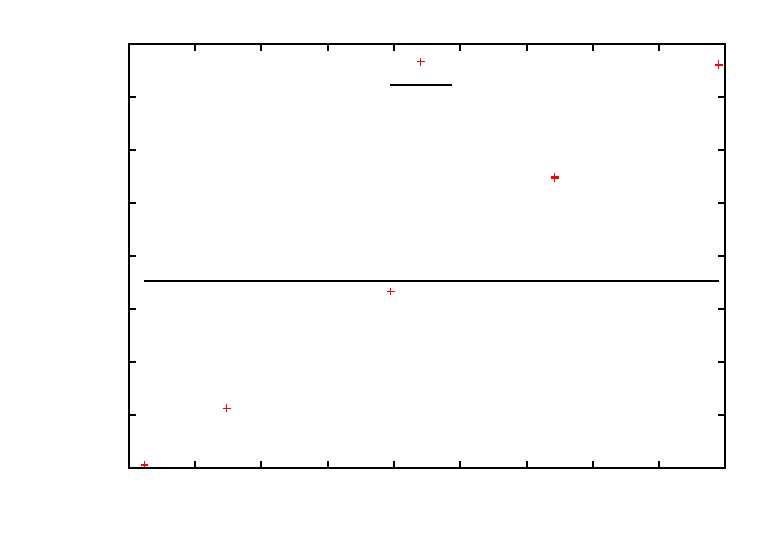
\includegraphics{Kalibration}}%
    \gplfronttext
  \end{picture}%
\endgroup

 \caption{Skalenteile des Messgeräts in Abhängigkeit der geflossenen Ladung}
 \label{fig:Kalibration}
\end{figure}

\subsection{Berechnung von $\varepsilon_0$}
Wir legen an den Kondensator eine Spannung an und lassen danach die aufgebrachte Ladung über das Ladungsmessgerät abfließen.
Mit folgender Formel kann dann die Kapazität berechnet werden.
\begin{align*}
	C&=\frac{Q}{U}\\
	\sigma_{C}&=\frac{1}{U^{2}} \cdot \sqrt{Q^{2} \cdot \sigma_{U}^{2} + \sigma_{Q}^{2} \cdot U^{2}}
\end{align*}

Mit einer angelegten Spannung $U=(220 \pm 0.1)\,$V und einer gemessenen Ladung $Q=\left(8.89 \pm 0.07\right) \cdot 10^{-7}\,\si{\coulomb}$ folgt für die Kapazität des Plattenkondensators
\begin{empheq}[box=\shadowbox*]{align}
	C&=\left(4.04 \pm 0.03\right)\, \si{\nano\farad}
\end{empheq}

Stellt man \eqref{eq:C_Pl} nun nach der elektrischen Feldkonstante $\varepsilon_0$ um und setzt die oben angegebenen Angaben des Plattenkondensators sowie die gemessene Kapazität ein, erhält man
\begin{empheq}[box=\shadowbox*]{align}
	\varepsilon_0= \left(9.19 \pm 0.07\right)\cdot 10^{-12}\,\si[per-mode=fraction]{\ampere\second\per\volt\per\meter}
\end{empheq}


\subsection{Entladung des Kondensators}
Trägt man die Ladung, die sich auf dem Plattenkondensator befindet und über einen Widerstand $R$ abfließt, logarithmisch gegen die Zeit auf (Abb. \ref{fig:R_iso} und \ref{fig:R_x+R_iso}), ergibt sich nach \eqref{eq:Q(t)} eine Gerade.
Aus der Geradensteigung $m$ kann mit dem obigen Ergebnis für die Kapazität der Widerstand $R$ berechnet werden.
\begin{align*}
	R&=- \frac{1}{C \cdot m}\\
	\sigma_{R}&=\frac{1}{C^{2} \cdot m^{2}} \cdot \sqrt{C^{2} \cdot \sigma_{m}^{2} + m^{2} \cdot \sigma_{C}^{2}}
\end{align*}

Setzt man nun die Geradensteigung $m_\text{iso}$ aus Abb.\ref{fig:R_iso} ein, erhält man für den Isolationswiderstand $R_\text{iso}$ des Plattenkondensators folgenden Wert:
\begin{empheq}[box=\shadowbox*]{align}
	R_\text{iso}&=\left(15 \pm 1\right)\, \si{\giga\ohm}
\end{empheq}

Analog wird der Gesamtwiderstand $R=\left(2.4 \pm 0.2\right) \, \si{\giga\ohm}$ aus der zweiten Messung berechnet.
Dieser setzt sich jedoch aus dem eben berechneten  Isolationswiderstand und dem unbekannten Widerstand $R_x$ zusammen, die parallel geschaltet sind.
\begin{align*}
	R_x&=\left(\frac{1}{R} - \frac{1}{R_\text{iso}}\right)^{-1}\\
	\sigma_{R_x}&=\frac{1}{\left(R_\text{iso} - R\right)^{2}} \cdot \sqrt{R_\text{iso}^{4} \cdot \sigma_{R}^{2} + R^{4} \cdot \sigma_{R_\text{iso}}^{2}}
\end{align*}
Es ergibt sich also:
\begin{empheq}[box=\shadowbox*]{align}
	R_x&=\left(2.8 \pm 0.4\right) \, \si{\giga\ohm}
\end{empheq}

\begin{figure}[!htb]
	\centering
	% GNUPLOT: LaTeX picture with Postscript
\begingroup
  \makeatletter
  \providecommand\color[2][]{%
    \GenericError{(gnuplot) \space\space\space\@spaces}{%
      Package color not loaded in conjunction with
      terminal option `colourtext'%
    }{See the gnuplot documentation for explanation.%
    }{Either use 'blacktext' in gnuplot or load the package
      color.sty in LaTeX.}%
    \renewcommand\color[2][]{}%
  }%
  \providecommand\includegraphics[2][]{%
    \GenericError{(gnuplot) \space\space\space\@spaces}{%
      Package graphicx or graphics not loaded%
    }{See the gnuplot documentation for explanation.%
    }{The gnuplot epslatex terminal needs graphicx.sty or graphics.sty.}%
    \renewcommand\includegraphics[2][]{}%
  }%
  \providecommand\rotatebox[2]{#2}%
  \@ifundefined{ifGPcolor}{%
    \newif\ifGPcolor
    \GPcolortrue
  }{}%
  \@ifundefined{ifGPblacktext}{%
    \newif\ifGPblacktext
    \GPblacktexttrue
  }{}%
  % define a \g@addto@macro without @ in the name:
  \let\gplgaddtomacro\g@addto@macro
  % define empty templates for all commands taking text:
  \gdef\gplbacktext{}%
  \gdef\gplfronttext{}%
  \makeatother
  \ifGPblacktext
    % no textcolor at all
    \def\colorrgb#1{}%
    \def\colorgray#1{}%
  \else
    % gray or color?
    \ifGPcolor
      \def\colorrgb#1{\color[rgb]{#1}}%
      \def\colorgray#1{\color[gray]{#1}}%
      \expandafter\def\csname LTw\endcsname{\color{white}}%
      \expandafter\def\csname LTb\endcsname{\color{black}}%
      \expandafter\def\csname LTa\endcsname{\color{black}}%
      \expandafter\def\csname LT0\endcsname{\color[rgb]{1,0,0}}%
      \expandafter\def\csname LT1\endcsname{\color[rgb]{0,1,0}}%
      \expandafter\def\csname LT2\endcsname{\color[rgb]{0,0,1}}%
      \expandafter\def\csname LT3\endcsname{\color[rgb]{1,0,1}}%
      \expandafter\def\csname LT4\endcsname{\color[rgb]{0,1,1}}%
      \expandafter\def\csname LT5\endcsname{\color[rgb]{1,1,0}}%
      \expandafter\def\csname LT6\endcsname{\color[rgb]{0,0,0}}%
      \expandafter\def\csname LT7\endcsname{\color[rgb]{1,0.3,0}}%
      \expandafter\def\csname LT8\endcsname{\color[rgb]{0.5,0.5,0.5}}%
    \else
      % gray
      \def\colorrgb#1{\color{black}}%
      \def\colorgray#1{\color[gray]{#1}}%
      \expandafter\def\csname LTw\endcsname{\color{white}}%
      \expandafter\def\csname LTb\endcsname{\color{black}}%
      \expandafter\def\csname LTa\endcsname{\color{black}}%
      \expandafter\def\csname LT0\endcsname{\color{black}}%
      \expandafter\def\csname LT1\endcsname{\color{black}}%
      \expandafter\def\csname LT2\endcsname{\color{black}}%
      \expandafter\def\csname LT3\endcsname{\color{black}}%
      \expandafter\def\csname LT4\endcsname{\color{black}}%
      \expandafter\def\csname LT5\endcsname{\color{black}}%
      \expandafter\def\csname LT6\endcsname{\color{black}}%
      \expandafter\def\csname LT7\endcsname{\color{black}}%
      \expandafter\def\csname LT8\endcsname{\color{black}}%
    \fi
  \fi
  \setlength{\unitlength}{0.0500bp}%
  \begin{picture}(7200.00,5040.00)%
    \gplgaddtomacro\gplbacktext{%
      \csname LTb\endcsname%
      \put(990,704){\makebox(0,0)[r]{\strut{}-6}}%
      \put(990,1383){\makebox(0,0)[r]{\strut{}-5}}%
      \put(990,2061){\makebox(0,0)[r]{\strut{}-4}}%
      \put(990,2740){\makebox(0,0)[r]{\strut{}-3}}%
      \put(990,3419){\makebox(0,0)[r]{\strut{}-2}}%
      \put(990,4097){\makebox(0,0)[r]{\strut{}-1}}%
      \put(990,4776){\makebox(0,0)[r]{\strut{} 0}}%
      \put(1122,484){\makebox(0,0){\strut{} 0}}%
      \put(2095,484){\makebox(0,0){\strut{} 50}}%
      \put(3067,484){\makebox(0,0){\strut{} 100}}%
      \put(4040,484){\makebox(0,0){\strut{} 150}}%
      \put(5013,484){\makebox(0,0){\strut{} 200}}%
      \put(5985,484){\makebox(0,0){\strut{} 250}}%
      \put(6958,484){\makebox(0,0){\strut{} 300}}%
      \put(484,2740){\rotatebox{90}{\makebox(0,0){\strut{}$\ln(Q/Q_0)$}}}%
      \put(4040,154){\makebox(0,0){\strut{}Zeit [s]}}%
    }%
    \gplgaddtomacro\gplfronttext{%
      \csname LTb\endcsname%
      \put(3498,4603){\makebox(0,0)[r]{\strut{}Messwerte}}%
      \csname LTb\endcsname%
      \put(3498,4383){\makebox(0,0)[r]{\strut{}Regressionsgerade}}%
    }%
    \gplbacktext
    \put(0,0){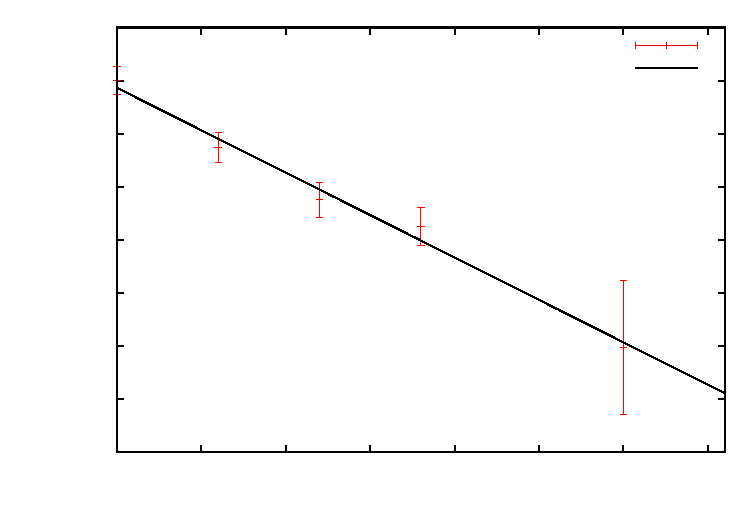
\includegraphics{Entladen2}}%
    \gplfronttext
  \end{picture}%
\endgroup

	\caption{Entladung des Kondesators über den Isolationswiderstand $R_\text{iso}$}
	\label{fig:R_iso}
\end{figure}

\begin{figure}[!htb]
	\centering
	% GNUPLOT: LaTeX picture with Postscript
\begingroup
  \makeatletter
  \providecommand\color[2][]{%
    \GenericError{(gnuplot) \space\space\space\@spaces}{%
      Package color not loaded in conjunction with
      terminal option `colourtext'%
    }{See the gnuplot documentation for explanation.%
    }{Either use 'blacktext' in gnuplot or load the package
      color.sty in LaTeX.}%
    \renewcommand\color[2][]{}%
  }%
  \providecommand\includegraphics[2][]{%
    \GenericError{(gnuplot) \space\space\space\@spaces}{%
      Package graphicx or graphics not loaded%
    }{See the gnuplot documentation for explanation.%
    }{The gnuplot epslatex terminal needs graphicx.sty or graphics.sty.}%
    \renewcommand\includegraphics[2][]{}%
  }%
  \providecommand\rotatebox[2]{#2}%
  \@ifundefined{ifGPcolor}{%
    \newif\ifGPcolor
    \GPcolortrue
  }{}%
  \@ifundefined{ifGPblacktext}{%
    \newif\ifGPblacktext
    \GPblacktexttrue
  }{}%
  % define a \g@addto@macro without @ in the name:
  \let\gplgaddtomacro\g@addto@macro
  % define empty templates for all commands taking text:
  \gdef\gplbacktext{}%
  \gdef\gplfronttext{}%
  \makeatother
  \ifGPblacktext
    % no textcolor at all
    \def\colorrgb#1{}%
    \def\colorgray#1{}%
  \else
    % gray or color?
    \ifGPcolor
      \def\colorrgb#1{\color[rgb]{#1}}%
      \def\colorgray#1{\color[gray]{#1}}%
      \expandafter\def\csname LTw\endcsname{\color{white}}%
      \expandafter\def\csname LTb\endcsname{\color{black}}%
      \expandafter\def\csname LTa\endcsname{\color{black}}%
      \expandafter\def\csname LT0\endcsname{\color[rgb]{1,0,0}}%
      \expandafter\def\csname LT1\endcsname{\color[rgb]{0,1,0}}%
      \expandafter\def\csname LT2\endcsname{\color[rgb]{0,0,1}}%
      \expandafter\def\csname LT3\endcsname{\color[rgb]{1,0,1}}%
      \expandafter\def\csname LT4\endcsname{\color[rgb]{0,1,1}}%
      \expandafter\def\csname LT5\endcsname{\color[rgb]{1,1,0}}%
      \expandafter\def\csname LT6\endcsname{\color[rgb]{0,0,0}}%
      \expandafter\def\csname LT7\endcsname{\color[rgb]{1,0.3,0}}%
      \expandafter\def\csname LT8\endcsname{\color[rgb]{0.5,0.5,0.5}}%
    \else
      % gray
      \def\colorrgb#1{\color{black}}%
      \def\colorgray#1{\color[gray]{#1}}%
      \expandafter\def\csname LTw\endcsname{\color{white}}%
      \expandafter\def\csname LTb\endcsname{\color{black}}%
      \expandafter\def\csname LTa\endcsname{\color{black}}%
      \expandafter\def\csname LT0\endcsname{\color{black}}%
      \expandafter\def\csname LT1\endcsname{\color{black}}%
      \expandafter\def\csname LT2\endcsname{\color{black}}%
      \expandafter\def\csname LT3\endcsname{\color{black}}%
      \expandafter\def\csname LT4\endcsname{\color{black}}%
      \expandafter\def\csname LT5\endcsname{\color{black}}%
      \expandafter\def\csname LT6\endcsname{\color{black}}%
      \expandafter\def\csname LT7\endcsname{\color{black}}%
      \expandafter\def\csname LT8\endcsname{\color{black}}%
    \fi
  \fi
  \setlength{\unitlength}{0.0500bp}%
  \begin{picture}(7200.00,5040.00)%
    \gplgaddtomacro\gplbacktext{%
      \csname LTb\endcsname%
      \put(990,704){\makebox(0,0)[r]{\strut{}-8}}%
      \put(990,1156){\makebox(0,0)[r]{\strut{}-7}}%
      \put(990,1609){\makebox(0,0)[r]{\strut{}-6}}%
      \put(990,2061){\makebox(0,0)[r]{\strut{}-5}}%
      \put(990,2514){\makebox(0,0)[r]{\strut{}-4}}%
      \put(990,2966){\makebox(0,0)[r]{\strut{}-3}}%
      \put(990,3419){\makebox(0,0)[r]{\strut{}-2}}%
      \put(990,3871){\makebox(0,0)[r]{\strut{}-1}}%
      \put(990,4324){\makebox(0,0)[r]{\strut{} 0}}%
      \put(990,4776){\makebox(0,0)[r]{\strut{} 1}}%
      \put(1122,484){\makebox(0,0){\strut{} 0}}%
      \put(1956,484){\makebox(0,0){\strut{} 10}}%
      \put(2789,484){\makebox(0,0){\strut{} 20}}%
      \put(3623,484){\makebox(0,0){\strut{} 30}}%
      \put(4457,484){\makebox(0,0){\strut{} 40}}%
      \put(5291,484){\makebox(0,0){\strut{} 50}}%
      \put(6124,484){\makebox(0,0){\strut{} 60}}%
      \put(6958,484){\makebox(0,0){\strut{} 70}}%
      \put(484,2740){\rotatebox{90}{\makebox(0,0){\strut{}$\ln(Q/Q_0)$}}}%
      \put(4040,154){\makebox(0,0){\strut{}Zeit [s]}}%
    }%
    \gplgaddtomacro\gplfronttext{%
      \csname LTb\endcsname%
      \put(5971,4603){\makebox(0,0)[r]{\strut{}Messwerte}}%
      \csname LTb\endcsname%
      \put(5971,4383){\makebox(0,0)[r]{\strut{}Regressionsgerade}}%
    }%
    \gplbacktext
    \put(0,0){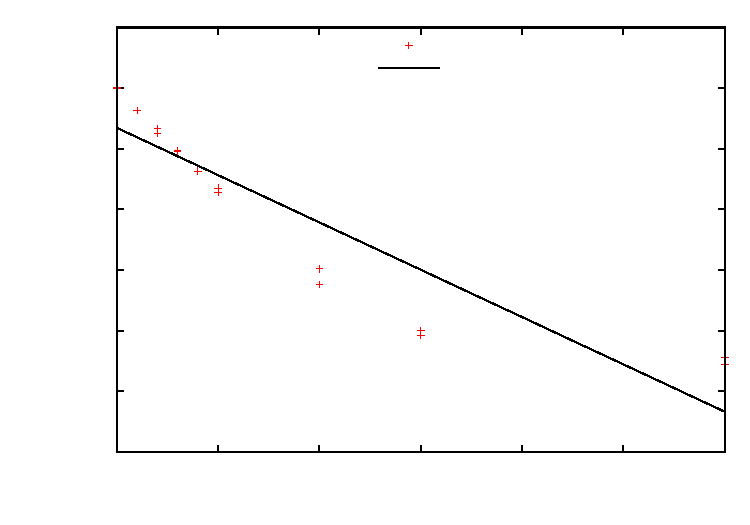
\includegraphics{Entladen1}}%
    \gplfronttext
  \end{picture}%
\endgroup

	\caption{Entladung des Kondesators über $R_x$ und $R_\text{iso}$}
	\label{fig:R_x+R_iso}
\end{figure}

\subsection{Messungen mit dem Oszilloskop}
Die ausgedruckten Spannungsverläufe befinden sich im Anhang.
Wie erwartet ergibt sich folgendes:
Bei RC-Schaltungen ergibt sich eine abfallende Exponentialfunktion.
Je größer der Widerstand bzw. die Kapazität, desto größer die Abfallzeit.
Bei den RLC-Kreisen ergibt sich eine abfallende Schwingung:
Je größer der Widerstand bzw. kleiner die Induktivität, desto schneller fällt die Einhüllende ab.
All dies wird in der nachfolgenden Auswertung verifiziert.  

\subsubsection{Eingangswiderstand des Oszilloskops und Kapazität des Plattenkondensators}
\begin{align*}
	R_\text{oszi}&=R_2 \cdot \left(\frac{m_\text{ges}}{m_\text{oszi}} - 1\right)\\
	\sigma_{R_\text{oszi}}&=\frac{1}{m_\text{oszi}^{2}} \cdot \sqrt{m_\text{ges}^{2} \cdot R_2^{2} \cdot \sigma_{m_\text{oszi}}^{2} + m_\text{oszi}^{2} \cdot \left(R_2^{2} \cdot \sigma_{m_\text{ges}}^{2} + \sigma_{R_2}^{2} \cdot \left(m_\text{ges} - m_\text{oszi}\right)^{2}\right)}
\end{align*}

\begin{empheq}[box=\shadowbox*]{align}
	R_\text{oszi}&=\left(900 \pm 60\right) \, \si{\kilo\ohm}
\end{empheq}

\begin{align*}
	C&=- \frac{1}{m_\text{oszi} \cdot R_\text{oszi}}\\
	\sigma_{C}&=\frac{1}{m_\text{oszi}^{2} \cdot R_\text{oszi}^{2}} \cdot \sqrt{m_\text{oszi}^{2} \cdot \sigma_{R_\text{oszi}}^{2} + R_\text{oszi}^{2} \cdot \sigma_{m_\text{oszi}}^{2}}
\end{align*}

\begin{empheq}[box=\shadowbox*]{align}
	C&=\left(4.3 \pm 0.3\right) \, \si{\nano\farad}
\end{empheq}


\subsubsection{Bestimmung des unbekannten Widerstandes $R_x$}
\begin{align*}
	R_x&=\frac{R_\text{oszi}}{\frac{m_x}{m_\text{oszi}} - 1}\\
	\sigma_{R_x}&=\frac{1}{\left(m_x - m_\text{oszi}\right)^{2}} \cdot \sqrt{m_\text{oszi}^{2} \cdot \sigma_{R_\text{oszi}}^{2} \cdot \left(m_x - m_\text{oszi}\right)^{2} + R_\text{oszi}^{2} \cdot \left(m_x^{2} \cdot \sigma_{m_\text{oszi}}^{2} + m_\text{oszi}^{2} \cdot \sigma_{m_x}^{2}\right)}
\end{align*}

\begin{empheq}[box=\shadowbox*]{align}
	R_x&=\left(-0.3 \pm 1.2\right) \, \si{\giga\ohm}
\end{empheq}


\subsubsection{Induktivität und ohmscher Widerstand der Spulen}
\begin{align*}
L&=\frac{T^{2}}{C \cdot \left(\beta^{2} \cdot T^{2} + 4 \cdot \pi^{2}\right)}\\
\sigma_{L}&=\frac{T}{C^{2} \cdot \left(\beta^{2} \cdot T^{2} + 4 \cdot \pi^{2}\right)^{2}} \cdot \sqrt{4 \cdot \beta^{2} \cdot C^{2} \cdot \sigma_{\beta}^{2} \cdot T^{6} + 64 \cdot \pi^{4} \cdot C^{2} \cdot \sigma_{T}^{2} + \sigma_{C}^{2} \cdot T^{2} \cdot \left(\beta^{2} \cdot T^{2} + 4 \cdot \pi^{2}\right)^{2}}
\end{align*}

\begin{align*}
	R_L&=2 \cdot \beta \cdot L\\
	\sigma_{R_L}&=2 \cdot \sqrt{\beta^{2} \cdot \sigma_{L}^{2} + L^{2} \cdot \sigma_{\beta}^{2}}
\end{align*}

Für die Drosselspule ergibt sich:	
\begin{empheq}[box=\shadowbox*]{align}
	L=(9.6 \pm 0.7)\, \si{\henry} \; , \;
	R_L=\left(6.1 \pm 0.5\right)\, \si{\kilo\ohm}
\end{empheq}
Für die Luftspule erhält man:
\begin{empheq}[box=\shadowbox*]{align}
	L=(0.018 \pm 0.001)\, \si{\henry} ~,~
	R_L=\left(160 \pm 10\right)\, \si{\ohm}
\end{empheq}

\subsubsection{Kapazität des Folienkondensators}
\begin{align*}
C_2&=\frac{C_\text{Pl.}}{m_g} \cdot m_c\\
\sigma_{C_2}&=\frac{1}{m_g^{2}} \cdot \sqrt{C_\text{Pl.}^{2} \cdot m_c^{2} \cdot \sigma_{m_g}^{2} + m_g^{2} \cdot \left(C_\text{Pl.}^{2} \cdot \sigma_{m_c}^{2} + m_c^{2} \cdot \sigma_{C_\text{Pl.}}^{2}\right)}
\end{align*}

\begin{empheq}[box=\shadowbox*]{align}
	C_2&=\left(3.1 \pm 0.2\right) \, \si{\nano\farad}
\end{empheq}


\section{Diskussion}
\label{sec:diskussion}

\section{Anhang}
\begin{figure}[!htb]
	\centering
	% GNUPLOT: LaTeX picture with Postscript
\begingroup
  \makeatletter
  \providecommand\color[2][]{%
    \GenericError{(gnuplot) \space\space\space\@spaces}{%
      Package color not loaded in conjunction with
      terminal option `colourtext'%
    }{See the gnuplot documentation for explanation.%
    }{Either use 'blacktext' in gnuplot or load the package
      color.sty in LaTeX.}%
    \renewcommand\color[2][]{}%
  }%
  \providecommand\includegraphics[2][]{%
    \GenericError{(gnuplot) \space\space\space\@spaces}{%
      Package graphicx or graphics not loaded%
    }{See the gnuplot documentation for explanation.%
    }{The gnuplot epslatex terminal needs graphicx.sty or graphics.sty.}%
    \renewcommand\includegraphics[2][]{}%
  }%
  \providecommand\rotatebox[2]{#2}%
  \@ifundefined{ifGPcolor}{%
    \newif\ifGPcolor
    \GPcolortrue
  }{}%
  \@ifundefined{ifGPblacktext}{%
    \newif\ifGPblacktext
    \GPblacktexttrue
  }{}%
  % define a \g@addto@macro without @ in the name:
  \let\gplgaddtomacro\g@addto@macro
  % define empty templates for all commands taking text:
  \gdef\gplbacktext{}%
  \gdef\gplfronttext{}%
  \makeatother
  \ifGPblacktext
    % no textcolor at all
    \def\colorrgb#1{}%
    \def\colorgray#1{}%
  \else
    % gray or color?
    \ifGPcolor
      \def\colorrgb#1{\color[rgb]{#1}}%
      \def\colorgray#1{\color[gray]{#1}}%
      \expandafter\def\csname LTw\endcsname{\color{white}}%
      \expandafter\def\csname LTb\endcsname{\color{black}}%
      \expandafter\def\csname LTa\endcsname{\color{black}}%
      \expandafter\def\csname LT0\endcsname{\color[rgb]{1,0,0}}%
      \expandafter\def\csname LT1\endcsname{\color[rgb]{0,1,0}}%
      \expandafter\def\csname LT2\endcsname{\color[rgb]{0,0,1}}%
      \expandafter\def\csname LT3\endcsname{\color[rgb]{1,0,1}}%
      \expandafter\def\csname LT4\endcsname{\color[rgb]{0,1,1}}%
      \expandafter\def\csname LT5\endcsname{\color[rgb]{1,1,0}}%
      \expandafter\def\csname LT6\endcsname{\color[rgb]{0,0,0}}%
      \expandafter\def\csname LT7\endcsname{\color[rgb]{1,0.3,0}}%
      \expandafter\def\csname LT8\endcsname{\color[rgb]{0.5,0.5,0.5}}%
    \else
      % gray
      \def\colorrgb#1{\color{black}}%
      \def\colorgray#1{\color[gray]{#1}}%
      \expandafter\def\csname LTw\endcsname{\color{white}}%
      \expandafter\def\csname LTb\endcsname{\color{black}}%
      \expandafter\def\csname LTa\endcsname{\color{black}}%
      \expandafter\def\csname LT0\endcsname{\color{black}}%
      \expandafter\def\csname LT1\endcsname{\color{black}}%
      \expandafter\def\csname LT2\endcsname{\color{black}}%
      \expandafter\def\csname LT3\endcsname{\color{black}}%
      \expandafter\def\csname LT4\endcsname{\color{black}}%
      \expandafter\def\csname LT5\endcsname{\color{black}}%
      \expandafter\def\csname LT6\endcsname{\color{black}}%
      \expandafter\def\csname LT7\endcsname{\color{black}}%
      \expandafter\def\csname LT8\endcsname{\color{black}}%
    \fi
  \fi
  \setlength{\unitlength}{0.0500bp}%
  \begin{picture}(7200.00,5040.00)%
    \gplgaddtomacro\gplbacktext{%
      \csname LTb\endcsname%
      \put(1254,704){\makebox(0,0)[r]{\strut{}-3.5}}%
      \put(1254,1111){\makebox(0,0)[r]{\strut{}-3}}%
      \put(1254,1518){\makebox(0,0)[r]{\strut{}-2.5}}%
      \put(1254,1926){\makebox(0,0)[r]{\strut{}-2}}%
      \put(1254,2333){\makebox(0,0)[r]{\strut{}-1.5}}%
      \put(1254,2740){\makebox(0,0)[r]{\strut{}-1}}%
      \put(1254,3147){\makebox(0,0)[r]{\strut{}-0.5}}%
      \put(1254,3554){\makebox(0,0)[r]{\strut{} 0}}%
      \put(1254,3962){\makebox(0,0)[r]{\strut{} 0.5}}%
      \put(1254,4369){\makebox(0,0)[r]{\strut{} 1}}%
      \put(1254,4776){\makebox(0,0)[r]{\strut{} 1.5}}%
      \put(1386,484){\makebox(0,0){\strut{} 0}}%
      \put(2315,484){\makebox(0,0){\strut{} 2}}%
      \put(3243,484){\makebox(0,0){\strut{} 4}}%
      \put(4172,484){\makebox(0,0){\strut{} 6}}%
      \put(5101,484){\makebox(0,0){\strut{} 8}}%
      \put(6029,484){\makebox(0,0){\strut{} 10}}%
      \put(6958,484){\makebox(0,0){\strut{} 12}}%
      \put(484,2740){\rotatebox{90}{\makebox(0,0){\strut{}$\ln(U)$}}}%
      \put(4172,154){\makebox(0,0){\strut{}Zeit [ms]}}%
    }%
    \gplgaddtomacro\gplfronttext{%
      \csname LTb\endcsname%
      \put(3762,4603){\makebox(0,0)[r]{\strut{}Messwerte}}%
      \csname LTb\endcsname%
      \put(3762,4383){\makebox(0,0)[r]{\strut{}Regressionsgerade}}%
    }%
    \gplbacktext
    \put(0,0){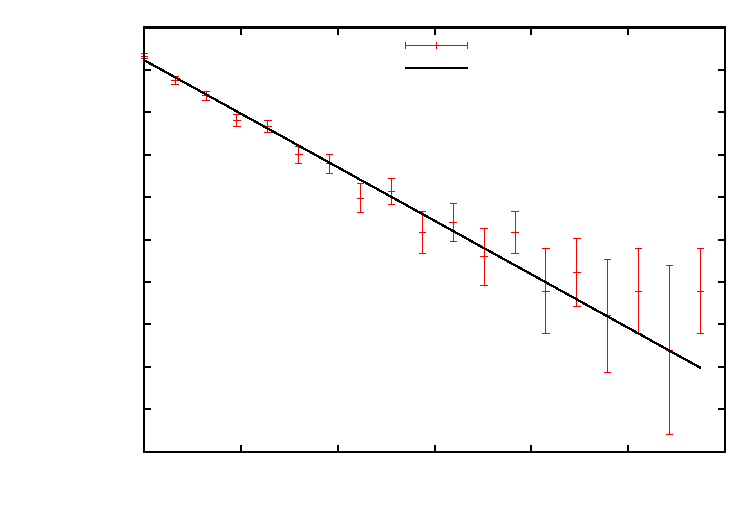
\includegraphics{Drosselspule}}%
    \gplfronttext
  \end{picture}%
\endgroup

	\caption{\textit{Drosselspule}: Extrema des Spannungsverlauf logarithmisch gegen die Zeit}
\end{figure}

\begin{figure}[!htb]
	\centering
	% GNUPLOT: LaTeX picture with Postscript
\begingroup
  \makeatletter
  \providecommand\color[2][]{%
    \GenericError{(gnuplot) \space\space\space\@spaces}{%
      Package color not loaded in conjunction with
      terminal option `colourtext'%
    }{See the gnuplot documentation for explanation.%
    }{Either use 'blacktext' in gnuplot or load the package
      color.sty in LaTeX.}%
    \renewcommand\color[2][]{}%
  }%
  \providecommand\includegraphics[2][]{%
    \GenericError{(gnuplot) \space\space\space\@spaces}{%
      Package graphicx or graphics not loaded%
    }{See the gnuplot documentation for explanation.%
    }{The gnuplot epslatex terminal needs graphicx.sty or graphics.sty.}%
    \renewcommand\includegraphics[2][]{}%
  }%
  \providecommand\rotatebox[2]{#2}%
  \@ifundefined{ifGPcolor}{%
    \newif\ifGPcolor
    \GPcolortrue
  }{}%
  \@ifundefined{ifGPblacktext}{%
    \newif\ifGPblacktext
    \GPblacktexttrue
  }{}%
  % define a \g@addto@macro without @ in the name:
  \let\gplgaddtomacro\g@addto@macro
  % define empty templates for all commands taking text:
  \gdef\gplbacktext{}%
  \gdef\gplfronttext{}%
  \makeatother
  \ifGPblacktext
    % no textcolor at all
    \def\colorrgb#1{}%
    \def\colorgray#1{}%
  \else
    % gray or color?
    \ifGPcolor
      \def\colorrgb#1{\color[rgb]{#1}}%
      \def\colorgray#1{\color[gray]{#1}}%
      \expandafter\def\csname LTw\endcsname{\color{white}}%
      \expandafter\def\csname LTb\endcsname{\color{black}}%
      \expandafter\def\csname LTa\endcsname{\color{black}}%
      \expandafter\def\csname LT0\endcsname{\color[rgb]{1,0,0}}%
      \expandafter\def\csname LT1\endcsname{\color[rgb]{0,1,0}}%
      \expandafter\def\csname LT2\endcsname{\color[rgb]{0,0,1}}%
      \expandafter\def\csname LT3\endcsname{\color[rgb]{1,0,1}}%
      \expandafter\def\csname LT4\endcsname{\color[rgb]{0,1,1}}%
      \expandafter\def\csname LT5\endcsname{\color[rgb]{1,1,0}}%
      \expandafter\def\csname LT6\endcsname{\color[rgb]{0,0,0}}%
      \expandafter\def\csname LT7\endcsname{\color[rgb]{1,0.3,0}}%
      \expandafter\def\csname LT8\endcsname{\color[rgb]{0.5,0.5,0.5}}%
    \else
      % gray
      \def\colorrgb#1{\color{black}}%
      \def\colorgray#1{\color[gray]{#1}}%
      \expandafter\def\csname LTw\endcsname{\color{white}}%
      \expandafter\def\csname LTb\endcsname{\color{black}}%
      \expandafter\def\csname LTa\endcsname{\color{black}}%
      \expandafter\def\csname LT0\endcsname{\color{black}}%
      \expandafter\def\csname LT1\endcsname{\color{black}}%
      \expandafter\def\csname LT2\endcsname{\color{black}}%
      \expandafter\def\csname LT3\endcsname{\color{black}}%
      \expandafter\def\csname LT4\endcsname{\color{black}}%
      \expandafter\def\csname LT5\endcsname{\color{black}}%
      \expandafter\def\csname LT6\endcsname{\color{black}}%
      \expandafter\def\csname LT7\endcsname{\color{black}}%
      \expandafter\def\csname LT8\endcsname{\color{black}}%
    \fi
  \fi
  \setlength{\unitlength}{0.0500bp}%
  \begin{picture}(7200.00,5040.00)%
    \gplgaddtomacro\gplbacktext{%
      \csname LTb\endcsname%
      \put(990,704){\makebox(0,0)[r]{\strut{}-5}}%
      \put(990,1286){\makebox(0,0)[r]{\strut{}-4}}%
      \put(990,1867){\makebox(0,0)[r]{\strut{}-3}}%
      \put(990,2449){\makebox(0,0)[r]{\strut{}-2}}%
      \put(990,3031){\makebox(0,0)[r]{\strut{}-1}}%
      \put(990,3613){\makebox(0,0)[r]{\strut{} 0}}%
      \put(990,4194){\makebox(0,0)[r]{\strut{} 1}}%
      \put(990,4776){\makebox(0,0)[r]{\strut{} 2}}%
      \put(1122,484){\makebox(0,0){\strut{} 0}}%
      \put(2289,484){\makebox(0,0){\strut{} 50}}%
      \put(3456,484){\makebox(0,0){\strut{} 100}}%
      \put(4624,484){\makebox(0,0){\strut{} 150}}%
      \put(5791,484){\makebox(0,0){\strut{} 200}}%
      \put(6958,484){\makebox(0,0){\strut{} 250}}%
      \put(484,2740){\rotatebox{90}{\makebox(0,0){\strut{}$\ln(U)$}}}%
      \put(4040,154){\makebox(0,0){\strut{}Zeit [$\mu$s]}}%
    }%
    \gplgaddtomacro\gplfronttext{%
      \csname LTb\endcsname%
      \put(3498,4603){\makebox(0,0)[r]{\strut{}Messwerte}}%
      \csname LTb\endcsname%
      \put(3498,4383){\makebox(0,0)[r]{\strut{}Regressionsgerade}}%
    }%
    \gplbacktext
    \put(0,0){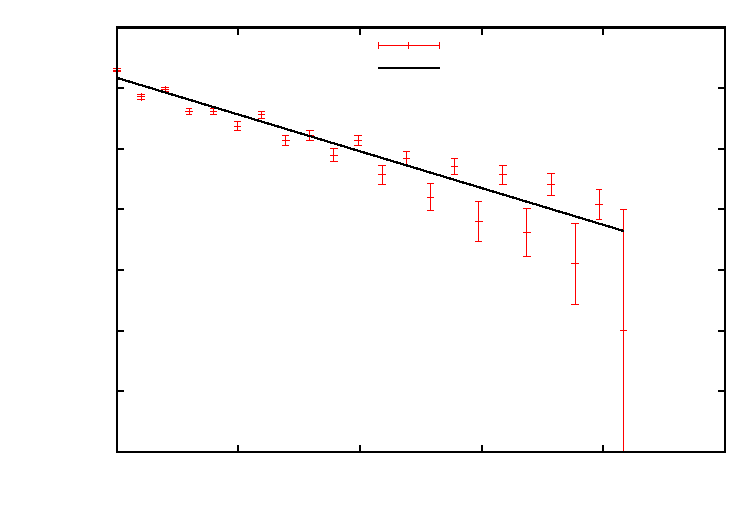
\includegraphics{Luftspule}}%
    \gplfronttext
  \end{picture}%
\endgroup

	\caption{\textit{Luftspule}: Extrema des Spannungsverlauf logarithmisch gegen die Zeit}
\end{figure}

\end{document}
